\documentclass[12pt,a4paper]{article}
% !TEX program = xelatex
\usepackage[utf8]{inputenc}
\usepackage[T1]{fontenc}
\usepackage[finnish]{babel}
\usepackage[utf8]{inputenc}
\usepackage{graphicx}
\usepackage{titling}
\usepackage{titlesec}
\usepackage{booktabs}
\usepackage{fancyhdr}
\usepackage{lipsum}
\usepackage{comment, mdframed}
\usepackage{enumitem}
\usepackage{xcolor}
\usepackage{longtable}
%\usepackage{cite}
\usepackage{pgfgantt}
\usepackage{amsmath, amssymb}
\usepackage{tikz}
\usepackage[margin=1in]{geometry}
\usepackage[backend=biber, style=numeric]{biblatex}
%\usepackage{hyperref}
\usepackage{bookmark}
\usepackage{enumitem}
\usepackage{amsmath}
\usepackage{listings}
\lstset{language=Python, basicstyle=\ttfamily\small, breaklines=true,columns=fullflexible}
\lstset{escapeinside={(*@}{@*)}}
\usepackage{fontspec}
\setmainfont{Arial}
\newfontfamily\stylishfont{Noteworthy}
%\newfontfamily\stylishfont{Zapfino}
%\addbibresource{references.bib}
\usetikzlibrary{calc}
\usepackage{xcolor}

\lstdefinestyle{pidstyle}{
    basicstyle=\ttfamily\footnotesize,
    breaklines=true,
    escapechar=\#, % Define escape character for inline LaTeX commands
    linewidth=\textwidth,
    basicstyle=\ttfamily\scriptsize
}

\renewcommand{\maketitle}{%
  \begin{leftmark}
    \vspace*{\baselineskip} % Add a bit of vertical space

%    \includegraphics[width=4cm]{example-image-a} % Add an image before the title. you will need to replace the image path with your own

%    \vspace{0.5cm} % Add vertical space before title

    \textbf{\fontsize{18}{36}\selectfont \thetitle} % Font Size and Bold Title

     \vspace{0.05cm} % Add vertical space before subtitle
%    \textit{\Large \theauthor}  % Subtitle / Author
    \vspace{\baselineskip} % Add vertical space after subtitle
     \rule{\textwidth}{0.4pt} % Add a horizontal line

   \end{leftmark}
%    \thispagestyle{empty} % Prevent header/footer on the title page
}


% Section Formatting
\titleformat{\section}
  {\normalfont\fontsize{18}{22}\bfseries} % Font and style
  {\thesection}         % Section number
  {1em}                   % Horizontal space after section number
  {}                     % Code before the section name
  []                     % Code after the section name

\titleformat{\subsection}
  {\normalfont\fontsize{14}{18}\bfseries} % Font and style
  {\thesubsection}         % Subsection number
  {1em}                   % Horizontal space after subsection number
  {}                     % Code before the subsection name
  []                     % Code after the subsection name

\setlength{\parindent}{0pt}

\title{Computing platforms (Spring 2025)\newline
week 6}
\author{Juha-Pekka Heikkilä}



\pagestyle{fancy}
\fancyhf{}

\renewcommand{\headrulewidth}{0pt}

\newcommand{\footerline}{\makebox[\textwidth]{\hrulefill}}

\newcommand{\footercontent}{%
    \begin{tabular}{@{}l@{}}
        \footerline \\
        \leftmark \hfill \rlap{\thepage}
    \end{tabular}
}

\fancyfoot[C]{\footercontent}


\newcommand{\exercise}[1]{
    \section*{Tehtävä #1}
    \markboth{Tehtävä #1}{}
}

\addtolength{\hoffset}{-1.75cm}
\addtolength{\textwidth}{3.5cm}
%\addtolength{\voffset}{-3cm}
%\addtolength{\textheight}{6cm}
%\setlength{\parindent}{0pt}



% (a), (b), (c)
\newlist{kohta}{enumerate}{1}
\setlist[kohta,1]{
  label=\textbf{\makebox[1cm][l]{\Huge\text{(\stylishfont\alph*)}}},
  leftmargin=!,
  labelindent=0pt
}

% (1), (2), (3)
\newlist{alakohta}{enumerate}{1}
\setlist[alakohta,1]{
  label=\textbf{\makebox[1cm][l]{\Large\text{(\arabic*)}}},
  leftmargin=!,
  labelindent=0pt
}

% termi: selitys
\newlist{kuvaus}{description}{1}
\setlist[kuvaus]{%
  font=\bfseries\stylishfont,
  labelsep=0.5cm,
  leftmargin=2.5cm,
  style=nextline
}

\newcommand{\korostus}[2][yellow]{\colorbox{#1}{\strut #2}}
%\korostus{Yksi kirjoittaja on jo sisällä}
%\korostus[red]{Lukijan täytyy odottaa jos kirjoittajia on paikalla}
%\korostus[orange]{Tämä osa ei ole suoritettavissa}


\newcommand{\evalslantti}[4][-12]{%
%  \left. #2 \,\right|% ei indeksejä tähän
  \mkern-10mu\raisebox{0pt}[0pt][0pt]{\rotatebox{#1}{$\Big|$}}% vinoviiva päälle
  \mkern3mu{}_{\!#3}^{\!#4}% arvot viivan oikealle puolelle
}


\newcommand{\evalraise}{1.2ex}
\newcommand{\evallow}{1.2ex}

% vino eval-viiva, arvot oikealla (oletus: -12)
% \evalslant[asteet]{lauseke}{ala}{yla}
\newcommand{\evalslant}[4][-12]{%
  \left. #2 \,\right.%
  \mkern-10mu\raisebox{0pt}[0pt][0pt]{\rotatebox{#1}{$\Big|$}}%
  \mkern2mu{}^{\raisebox{\evalraise}{$\scriptstyle #4$}}_{\raisebox{-\evallow}{$\scriptstyle #3$}}%
}



% vino eval-viiva ENNEN lauseketta
% \evalslantpre[asteet]{lauseke}{ala}{yla}
\newcommand{\evalslantpre}[4][-12]{%
  % viiva ja rajat
  \raisebox{0pt}[0pt][0pt]{\rotatebox{#1}{$\Big|$}}%
  \mkern2mu{}^{\raisebox{\evalraise}{$\scriptstyle #4$}}_{\raisebox{-\evallow}{$\scriptstyle #3$}}%
  % itse lauseke
  \mkern4mu\left. #2 \right.%
}


\DeclareMathOperator{\Var}{Var}
\DeclareMathOperator{\Cov}{Cov}
\DeclareMathOperator{\Corr}{Corr}
\usepackage{tikz}
\usetikzlibrary{automata, positioning, arrows}

\newcommand{\set}[1]{\left\{\,#1\,\right\}}
\newcommand{\abs}[1]{\lvert#1\rvert}

\newcommand{\N}{\mathbb{N}}
\newcommand{\Pot}{{\cal P}}

\newcommand{\rma}{\mathrm{a}}
\newcommand{\rmb}{\mathrm{b}}
\newcommand{\rmc}{\mathrm{c}}

\title{TKT20005 Laskennan mallit Viikko3}
\date{}

\begin{document}

\maketitle

\exercise{1 Äärellisen automaatin muodostaminen.} Tässä tehtävässä harjoitellaan muodostamaan äärellinen automaatti annetulle kielelle.
\begin{kohta}
\item
Piirrä deterministinen äärellinen automaatti, joka hyväksyy
tasan ne aakkoston $\set{\mathrm{a},\mathrm{b},\mathrm{c}}$
merkkijonot, jotka päättyvät cba.
\begin{center}
  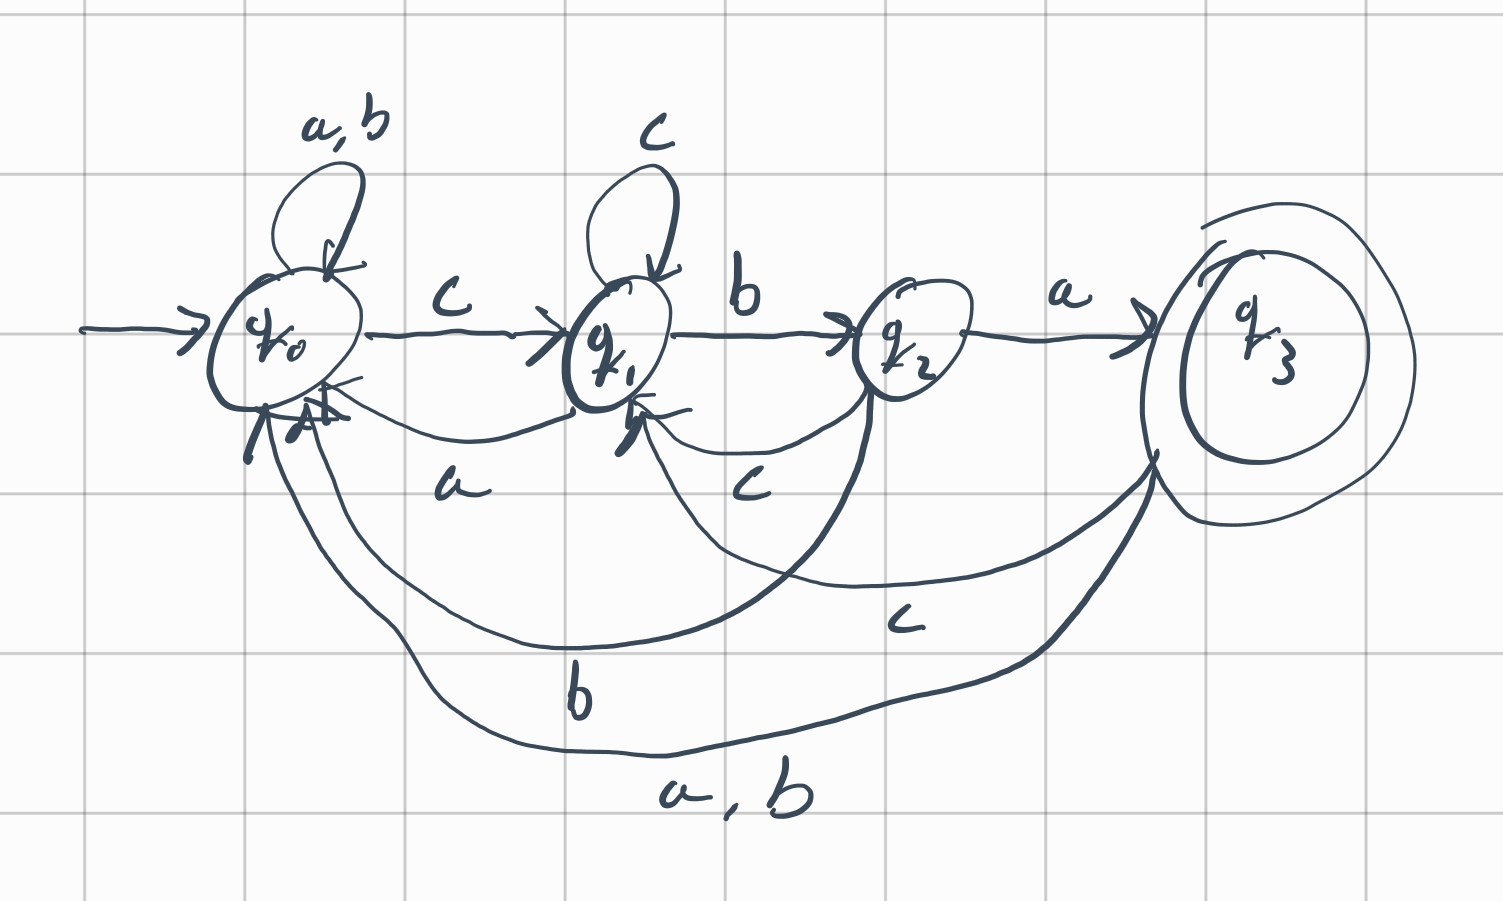
\includegraphics[width=.6\textwidth]{viikko3tehtävä1a.jpg}
\end{center}

\item
Piirrä deterministinen äärellinen automaatti, joka hyväksyy tasan ne 
aakkoston $\set{\mathrm{a},\mathrm{b},\mathrm{c}}$ merkkijonot,
jotka eivät sisällä osamerkkijonoa bc.\\
\begin{center}
  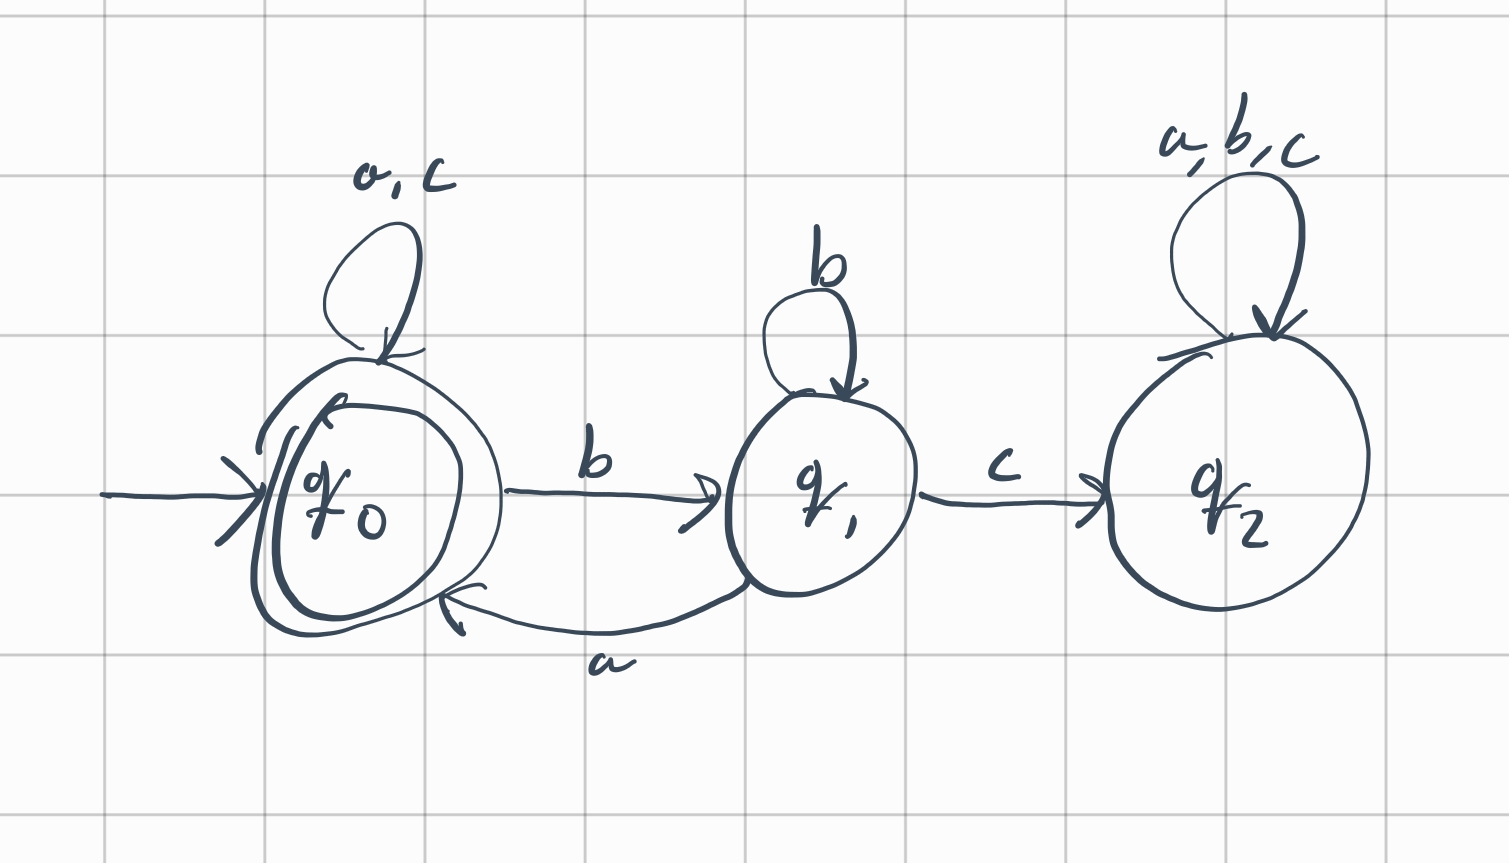
\includegraphics[width=.6\textwidth]{viikko3tehtävä1b.jpg}
\end{center}

\item
Piirrä deterministinen äärellinen automaatti, joka hyväksyy tasan ne 
aakkoston $\set{\mathrm{a},\mathrm{b},\mathrm{c}}$ merkkijonot,
joissa jokainen paritonnumeroinen merkki on b.
\begin{center}
  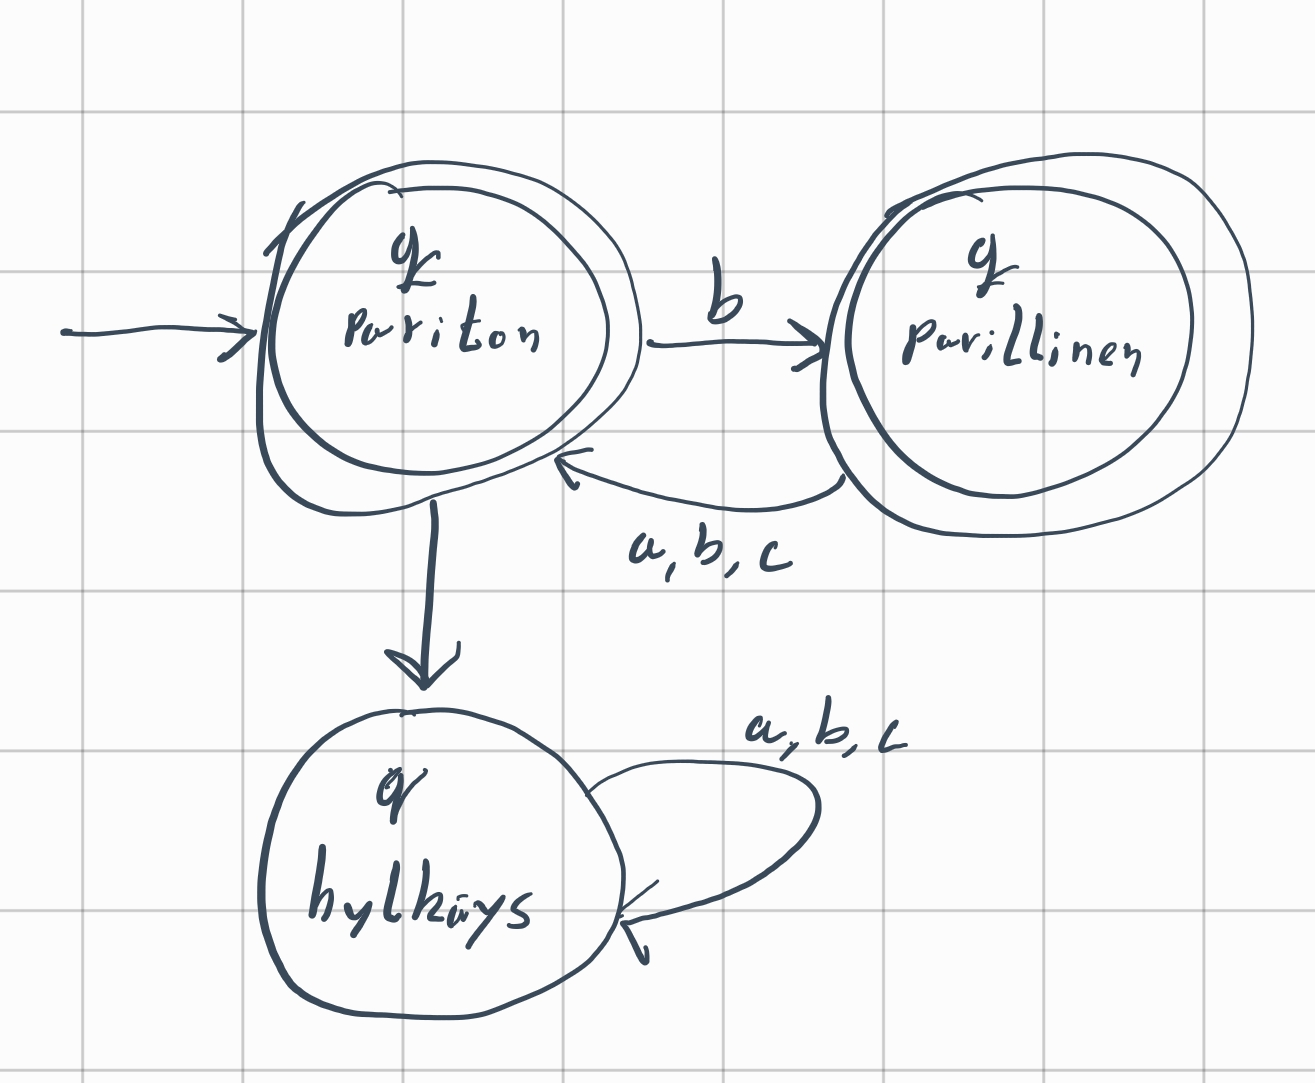
\includegraphics[width=.6\textwidth]{viikko3tehtävä1c.jpg}
\end{center}
Automaatti seuraa ollaanko lukemassa paritonta vai parillista merkkiä jonossa.

\item
Piirrä deterministinen äärellinen automaatti, joka hyväksyy tasan ne 
aakkoston $\set{\mathrm{a},\mathrm{b},\mathrm{c}}$ merkkijonot,
joissa a- ja b-merkkien lukumäärien erotus on
pariton.
\begin{center}
  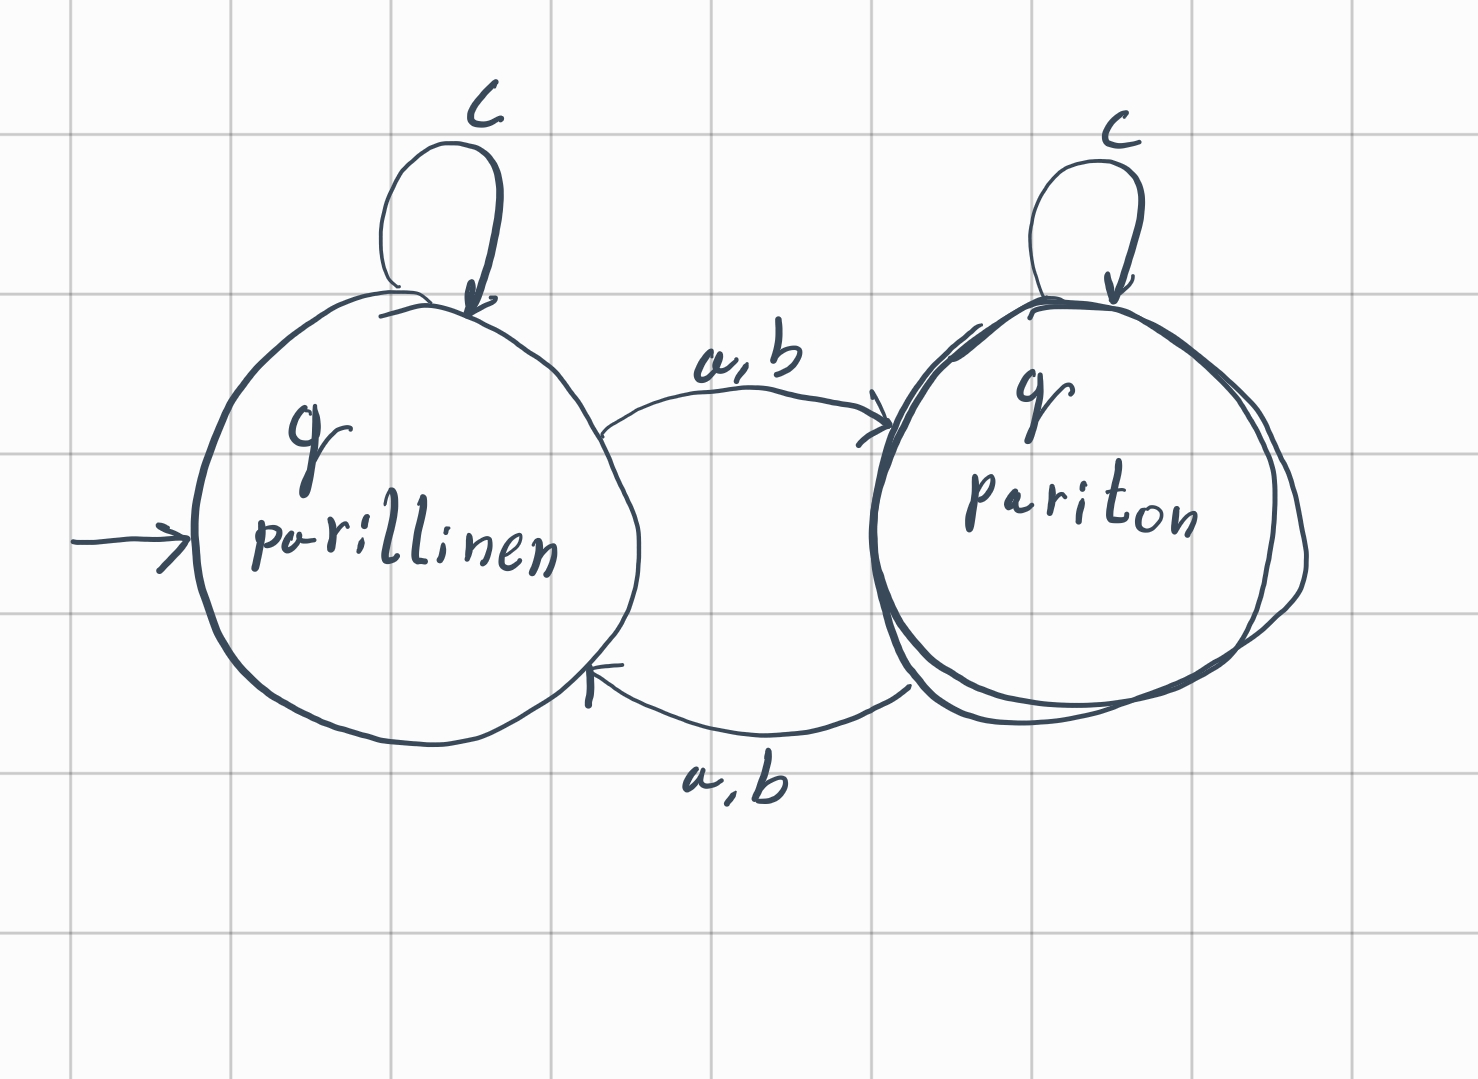
\includegraphics[width=.6\textwidth]{viikko3tehtävä1d.jpg}
\end{center}
'c' lukumäärä ei vaikuta. $|N_a - N_b|$ on pariton jos summa $N_a + N_b$
on pariton. Voidaan siis seurata a- ja b-merkkien yhteismäärän pariteettia.

\end{kohta}








\pagebreak
\exercise{2. Muunnos epädeterministisestä automaatista deterministiseksi.}

\begin{alakohta}
\item \textbf{NFA $\to$ DFA}

DFA alku on $\{1\}$. Hyväksyviä ovat osajoukot missä on $4$

\medskip
\noindent Siirtymätaulukko:
\[
\begin{array}{c|cc}
\text{\sigma} & a & b \\\hline
\{1\}   & \{2,4\} & \{2,4\} \\
\{2,4\} & \varnothing & \{1,3\} \\
\{1,3\} & \{2,4\} & \{2,4\} \\
\varnothing & \varnothing & \varnothing
\end{array}
\]


Hyväksyvä: $\{2,4\}$. Alkutila: $\{1\}$.

\begin{center}
  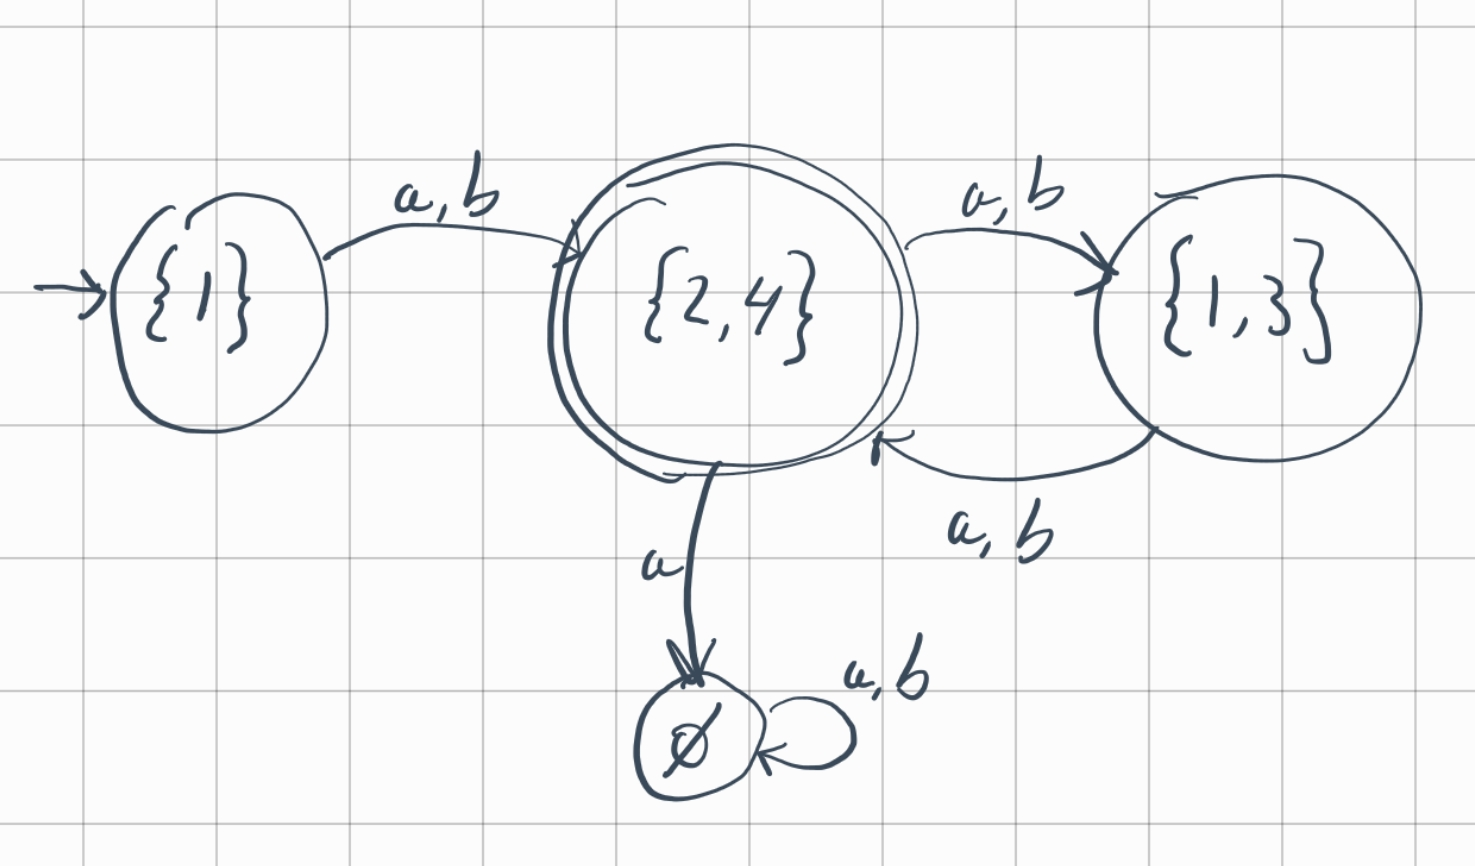
\includegraphics[width=.5\textwidth]{viikko3tehtävä21.jpg}
\end{center}


\item \textbf{Voiko DFA:ta yksinkertaistaa?} \\
Kyllä. \{1\} ja \{1,3\} kummastakin a ja b vievät aina samaan
tilaan \{2,4\}, ja kumpikaan ei ole hyväksyvä
jolloin ne voidaan yhdistää.

\medskip
\noindent Minimoitu siirtymätaulukko
\[
\begin{array}{c|cc}
\text{\sigma} & a & b \\\hline
S\ (\{1\}\!=\!\{1,3\}) & T & T \\
T\ (\{2,4\}) & D & S \\
D\ (\varnothing) & D & D
\end{array}
\]
Alku S (ei-hyväksyvä), hyväksyvä T, D on ikiluuppi.

\begin{center}
  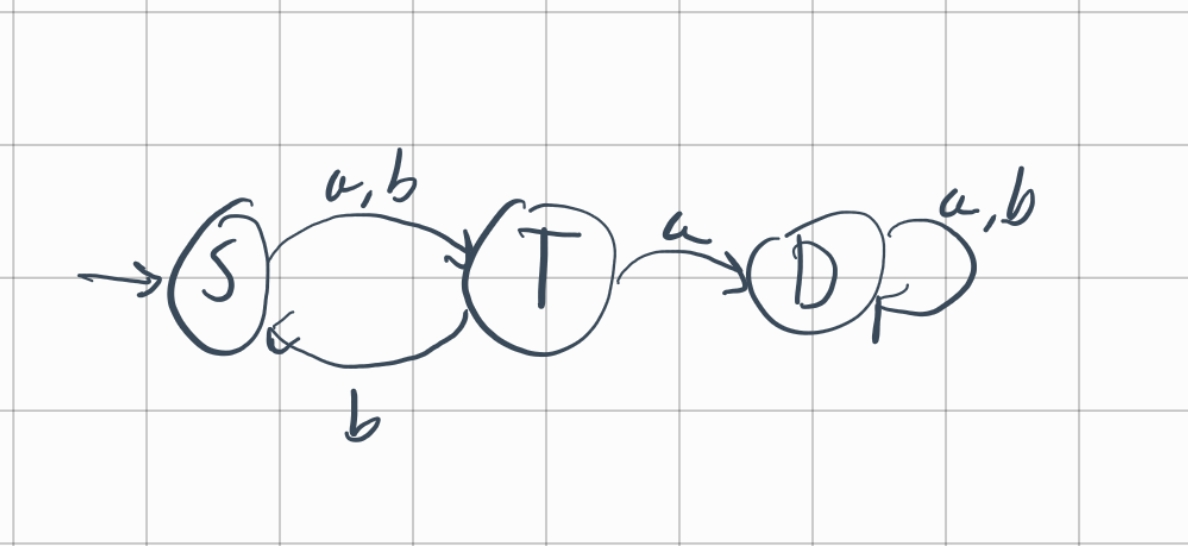
\includegraphics[width=.5\textwidth]{viikko3tehtävä22.jpg}
\end{center}

\end{alakohta}

\end{document}